\documentclass[border=4pt]{standalone}
\usepackage{tikz}
\usetikzlibrary{positioning, arrows.meta, calc, fit}
\begin{document}
	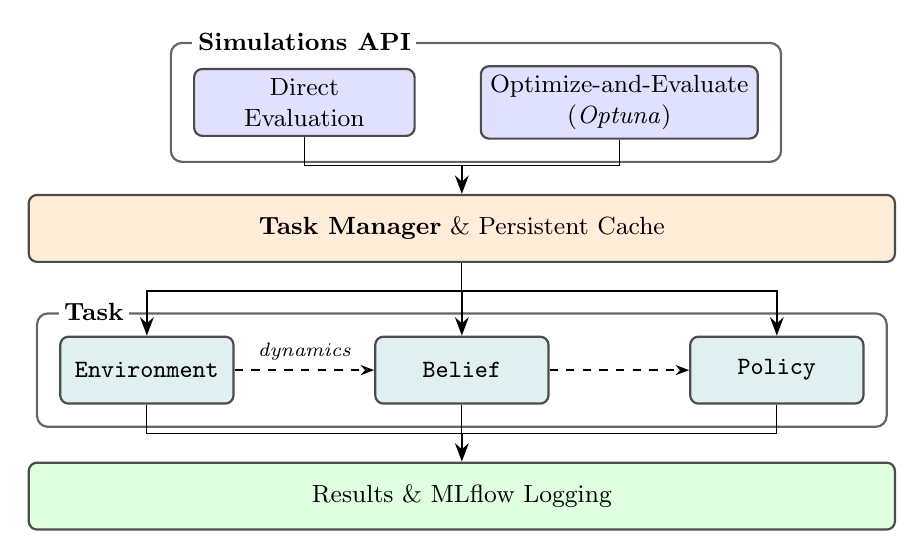
\begin{tikzpicture}[
	  wf/.style  = {rectangle, rounded corners=3pt, draw=black!70, thick,
	                fill=blue!12, minimum width=2.8cm, minimum height=0.85cm,
	                align=center, font=\small},
	  tm/.style  = {rectangle, rounded corners=3pt, draw=black!70, thick,
	                fill=orange!15, minimum width=11cm, minimum height=0.85cm,
	                align=center, font=\small},
	  ab/.style  = {rectangle, rounded corners=3pt, draw=black!70, thick,
	                fill=teal!12, minimum width=2.2cm, minimum height=0.85cm,
	                align=center, font=\small},
	  res/.style = {rectangle, rounded corners=3pt, draw=black!70, thick,
	                fill=green!12, minimum width=11cm, minimum height=0.85cm,
	                align=center, font=\small},
	  arr/.style = {-{Stealth[scale=1.0]}, thick},
	  int/.style = {-{Stealth[scale=0.85]}, dashed, semithick},
	  group/.style = {rectangle, rounded corners=4pt, draw=black!60,
	                  thick, inner sep=8pt},
	]
	% Row 1: Workflows
	\node[wf] (wf1) at (0.5,  0)    {Direct\\Evaluation};
	\node[wf] (wf2) at (4.5,  0)    {Optimize-and-Evaluate\\(\textit{Optuna})};
	% Row 2: Task Manager (centered at x=2.5)
	\node[tm] (tm)  at (2.5, -1.6)  {\textbf{Task Manager} \& Persistent Cache};
	% Row 3: Core Abstractions
	\node[ab] (env)    at (-1.5, -3.4) {\texttt{Environment}};
	\node[ab] (belief) at (2.5,  -3.4) {\texttt{Belief}};
	\node[ab] (policy) at (6.5,  -3.4) {\texttt{Policy}};
	% Row 4: Results
	\node[res] (out) at (2.5, -5.0)  {Results \& MLflow Logging};
	% Group workflows and the components of an episode task.
	\node[group, fit=(wf1)(wf2)] (api) {};
	\node[anchor=west, fill=white, inner sep=2pt, font=\small\bfseries]
	  at ([xshift=8pt]api.north west) {Simulations API};
	\node[group, fit=(env)(belief)(policy)] (task) {};
	\node[anchor=west, fill=white, inner sep=2pt, font=\small\bfseries]
	  at ([xshift=8pt]task.north west) {Task};
	% Junction coordinates
	\coordinate (jtm)  at (2.5, -0.8);
	\coordinate (jtb)  at (2.5, -2.4);
	\coordinate (jout) at (2.5, -4.2);
	% Workflows -> Task Manager (Y-junction)
	\draw      (wf1.south) |- (jtm);
	\draw      (wf2.south) |- (jtm);
	\draw[arr] (jtm) -- (tm.north);
	% Task Manager -> Core Abstractions (fork)
	\draw      (tm.south) -- (jtb);
	\draw[arr] (jtb) -| (env.north);
	\draw[arr] (jtb) -- (belief.north);
	\draw[arr] (jtb) -| (policy.north);
	% Interactions between abstractions (directional, dashed)
	\draw[int] (env.east)    -- node[above, font=\scriptsize\itshape] {dynamics} (belief.west);
	\draw[int] (belief.east) -- (policy.west);
	% Core Abstractions -> Results (Y-junction)
	\draw      (env.south)    |- (jout);
	\draw      (belief.south) -- (jout);
	\draw      (policy.south) |- (jout);
	\draw[arr] (jout) -- (out.north);
	\end{tikzpicture}
\end{document}
